\begin{frame}[allowframebreaks]
	\frametitle{Rascunho}
	\par Spiking Neural Networks (SNN) mimic how the brain works i.e. works with action potential in opposition to the continuous values crossing the links between the neurons. So, the more we understand the SNNs the more we understand the brains iteself.
	
	\par The "Spiking" comes from the behavior of the biological neuron which fires (action potential) from time to time creating voltage spikes when measured, these spikes represent the information \cite{kasabov2019time}. The figure \ref{fig:neuronspikes} shows the spikes.
	
	\begin{figure}
		\centering
		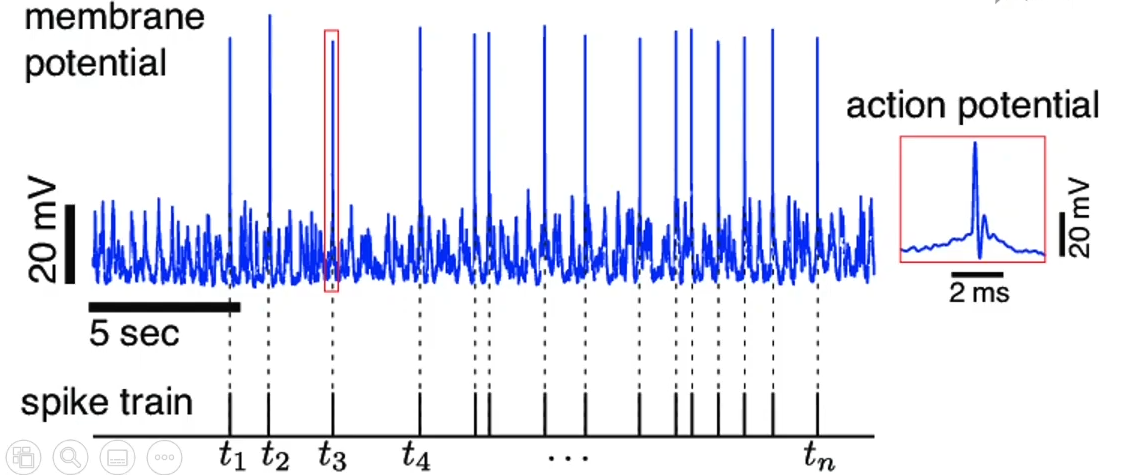
\includegraphics[width=0.6\linewidth]{images/neuronSpikes}
		\caption{Spikes from noisy signal. Source \cite{dan_goodman_2022_7044500}}
		\label{fig:neuronspikes}
	\end{figure}

	\par Spiking Neural Networks (SNNs) exhibit several noteworthy characteristics that set them apart from traditional machine learning techniques, including classical neural networks. These distinctions encompass \cite{kasabov2019time}:
	
	\begin{itemize}
		\item Proficiency in modeling temporal, spatio-temporal, or spectro-temporal data.
		\item Effectiveness in capturing processes involving various time scales.
		\item Seamless integration of multiple modalities, such as sound and vision, into a unified system.
		\item Aptitude for predictive modeling and event prediction.
		\item Swift and highly parallel information processing capabilities.
		\item Streamlined information processing.
		\item Scalability, accommodating structures ranging from a few tens to billions of spiking neurons.
		\item Minimal energy consumption when implemented on neuromorphic platforms.
	\end{itemize}

	\par In order to mimic such behavior let's begin with a simple model: The "Leaky Integrate and Fire neuron" (LIF). LIF evolves the membrane potential according to the equations bellow.
	
	\par Here we have the "leaking" equation which models the potencial losing across the time.
	\begin{equation}
		\tau . \dfrac{dV}{dt} = -V
		\label{eq:leak}
	\end{equation}
	
	\par When a neuron receives a spike V increases according to a synaptic weight w.
	\begin{equation}
		V = V + w
	\end{equation}


	\begin{figure}
		\centering
		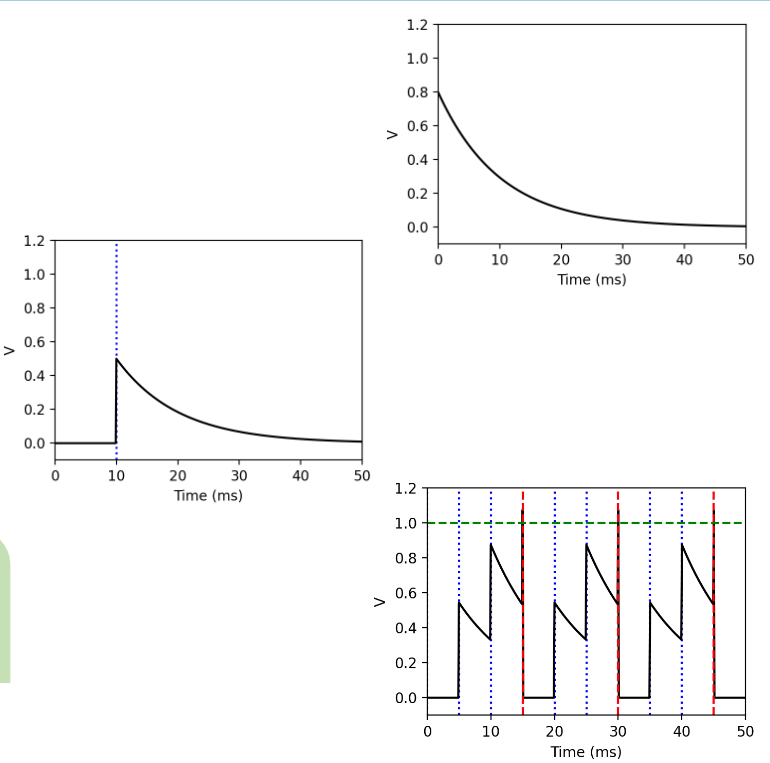
\includegraphics[width=0.5\linewidth]{images/neuronSpikes2}
		\caption{Evolution of a Spike. Source \cite{dan_goodman_2022_7044500}}
		\label{fig:neuronspikes2}
	\end{figure}

	\par Like it can be seen in Figure \ref{fig:neuronspikes2} when a neuron reaches some threshold it resets (V = 0) and starts an refractory period.
	
	\par Energy efficiency:
	
	\par Spiking Neural Networks (SNNs) are often considered power-efficient for several reasons:
	
	\begin{enumerate}
		\item Event-Driven Processing: SNNs are inherently event-driven. Instead of constantly updating neuron activations and synapse weights as in traditional artificial neural networks (ANNs), SNNs only transmit spikes (action potentials) when a neuron's membrane potential reaches a certain threshold. This event-driven approach reduces the amount of computation required and can lead to significant energy savings.
	
		\item Sparse Activity: SNNs tend to exhibit sparse activity, meaning that only a small percentage of neurons are active at any given time. This sparsity reduces the number of computations that need to be performed, which is especially beneficial for hardware implementations where most of the energy consumption comes from active components.
	
		\item Low Precision: SNNs can often work with lower precision than ANNs. While ANNs typically use high-precision floating-point numbers for neuron activations and synaptic weights, SNNs can use lower precision fixed-point or binary representations. Lower precision computations require less energy to perform.
	
		\item Neuromorphic Hardware: SNNs can be efficiently implemented on specialized neuromorphic hardware, which is designed to mimic the energy-efficient behavior of biological neural systems. These hardware platforms are optimized for the event-driven nature of SNNs, further reducing power consumption.
	
		\item Energy-Aware Learning Rules: SNNs can employ learning rules that take into account energy efficiency. For example, some learning rules prioritize strengthening or weakening synapses based on their contribution to network activity, which can lead to more energy-efficient learning.
	
		\item Spike Encoding: SNNs can encode information in the timing and frequency of spikes, which can be a highly efficient way to represent and process data, particularly for event-based sensors like vision sensors or auditory sensors.
	\end{enumerate}

	
		 
\end{frame}